\documentclass[11pt,]{article}
\usepackage{lmodern}
\usepackage{amssymb,amsmath}
\usepackage{ifxetex,ifluatex}
\usepackage{fixltx2e} % provides \textsubscript
\ifnum 0\ifxetex 1\fi\ifluatex 1\fi=0 % if pdftex
  \usepackage[T1]{fontenc}
  \usepackage[utf8]{inputenc}
\else % if luatex or xelatex
  \ifxetex
    \usepackage{mathspec}
  \else
    \usepackage{fontspec}
  \fi
  \defaultfontfeatures{Ligatures=TeX,Scale=MatchLowercase}
\fi
% use upquote if available, for straight quotes in verbatim environments
\IfFileExists{upquote.sty}{\usepackage{upquote}}{}
% use microtype if available
\IfFileExists{microtype.sty}{%
\usepackage{microtype}
\UseMicrotypeSet[protrusion]{basicmath} % disable protrusion for tt fonts
}{}
\usepackage[margin=1in]{geometry}
\usepackage{hyperref}
\PassOptionsToPackage{usenames,dvipsnames}{color} % color is loaded by hyperref
\hypersetup{unicode=true,
            pdftitle={Combining scientific data processing and publication using Literate Programming to enable reproducible research},
            pdfauthor={Andy Clifton},
            colorlinks=true,
            linkcolor=blue,
            citecolor=cyan,
            urlcolor=red,
            breaklinks=true}
\urlstyle{same}  % don't use monospace font for urls
\usepackage{natbib}
\bibliographystyle{plainnat}
\usepackage{color}
\usepackage{fancyvrb}
\newcommand{\VerbBar}{|}
\newcommand{\VERB}{\Verb[commandchars=\\\{\}]}
\DefineVerbatimEnvironment{Highlighting}{Verbatim}{commandchars=\\\{\}}
% Add ',fontsize=\small' for more characters per line
\usepackage{framed}
\definecolor{shadecolor}{RGB}{248,248,248}
\newenvironment{Shaded}{\begin{snugshade}}{\end{snugshade}}
\newcommand{\AlertTok}[1]{\textcolor[rgb]{0.94,0.16,0.16}{#1}}
\newcommand{\AnnotationTok}[1]{\textcolor[rgb]{0.56,0.35,0.01}{\textbf{\textit{#1}}}}
\newcommand{\AttributeTok}[1]{\textcolor[rgb]{0.77,0.63,0.00}{#1}}
\newcommand{\BaseNTok}[1]{\textcolor[rgb]{0.00,0.00,0.81}{#1}}
\newcommand{\BuiltInTok}[1]{#1}
\newcommand{\CharTok}[1]{\textcolor[rgb]{0.31,0.60,0.02}{#1}}
\newcommand{\CommentTok}[1]{\textcolor[rgb]{0.56,0.35,0.01}{\textit{#1}}}
\newcommand{\CommentVarTok}[1]{\textcolor[rgb]{0.56,0.35,0.01}{\textbf{\textit{#1}}}}
\newcommand{\ConstantTok}[1]{\textcolor[rgb]{0.00,0.00,0.00}{#1}}
\newcommand{\ControlFlowTok}[1]{\textcolor[rgb]{0.13,0.29,0.53}{\textbf{#1}}}
\newcommand{\DataTypeTok}[1]{\textcolor[rgb]{0.13,0.29,0.53}{#1}}
\newcommand{\DecValTok}[1]{\textcolor[rgb]{0.00,0.00,0.81}{#1}}
\newcommand{\DocumentationTok}[1]{\textcolor[rgb]{0.56,0.35,0.01}{\textbf{\textit{#1}}}}
\newcommand{\ErrorTok}[1]{\textcolor[rgb]{0.64,0.00,0.00}{\textbf{#1}}}
\newcommand{\ExtensionTok}[1]{#1}
\newcommand{\FloatTok}[1]{\textcolor[rgb]{0.00,0.00,0.81}{#1}}
\newcommand{\FunctionTok}[1]{\textcolor[rgb]{0.00,0.00,0.00}{#1}}
\newcommand{\ImportTok}[1]{#1}
\newcommand{\InformationTok}[1]{\textcolor[rgb]{0.56,0.35,0.01}{\textbf{\textit{#1}}}}
\newcommand{\KeywordTok}[1]{\textcolor[rgb]{0.13,0.29,0.53}{\textbf{#1}}}
\newcommand{\NormalTok}[1]{#1}
\newcommand{\OperatorTok}[1]{\textcolor[rgb]{0.81,0.36,0.00}{\textbf{#1}}}
\newcommand{\OtherTok}[1]{\textcolor[rgb]{0.56,0.35,0.01}{#1}}
\newcommand{\PreprocessorTok}[1]{\textcolor[rgb]{0.56,0.35,0.01}{\textit{#1}}}
\newcommand{\RegionMarkerTok}[1]{#1}
\newcommand{\SpecialCharTok}[1]{\textcolor[rgb]{0.00,0.00,0.00}{#1}}
\newcommand{\SpecialStringTok}[1]{\textcolor[rgb]{0.31,0.60,0.02}{#1}}
\newcommand{\StringTok}[1]{\textcolor[rgb]{0.31,0.60,0.02}{#1}}
\newcommand{\VariableTok}[1]{\textcolor[rgb]{0.00,0.00,0.00}{#1}}
\newcommand{\VerbatimStringTok}[1]{\textcolor[rgb]{0.31,0.60,0.02}{#1}}
\newcommand{\WarningTok}[1]{\textcolor[rgb]{0.56,0.35,0.01}{\textbf{\textit{#1}}}}
\usepackage{longtable,booktabs}
\usepackage{graphicx,grffile}
\makeatletter
\def\maxwidth{\ifdim\Gin@nat@width>\linewidth\linewidth\else\Gin@nat@width\fi}
\def\maxheight{\ifdim\Gin@nat@height>\textheight\textheight\else\Gin@nat@height\fi}
\makeatother
% Scale images if necessary, so that they will not overflow the page
% margins by default, and it is still possible to overwrite the defaults
% using explicit options in \includegraphics[width, height, ...]{}
\setkeys{Gin}{width=\maxwidth,height=\maxheight,keepaspectratio}
\IfFileExists{parskip.sty}{%
\usepackage{parskip}
}{% else
\setlength{\parindent}{0pt}
\setlength{\parskip}{6pt plus 2pt minus 1pt}
}
\setlength{\emergencystretch}{3em}  % prevent overfull lines
\providecommand{\tightlist}{%
  \setlength{\itemsep}{0pt}\setlength{\parskip}{0pt}}
\setcounter{secnumdepth}{5}
% Redefines (sub)paragraphs to behave more like sections
\ifx\paragraph\undefined\else
\let\oldparagraph\paragraph
\renewcommand{\paragraph}[1]{\oldparagraph{#1}\mbox{}}
\fi
\ifx\subparagraph\undefined\else
\let\oldsubparagraph\subparagraph
\renewcommand{\subparagraph}[1]{\oldsubparagraph{#1}\mbox{}}
\fi

%%% Use protect on footnotes to avoid problems with footnotes in titles
\let\rmarkdownfootnote\footnote%
\def\footnote{\protect\rmarkdownfootnote}

%%% Change title format to be more compact
\usepackage{titling}

% Create subtitle command for use in maketitle
\providecommand{\subtitle}[1]{
  \posttitle{
    \begin{center}\large#1\end{center}
    }
}

\setlength{\droptitle}{-2em}

  \title{Combining scientific data processing and publication using Literate Programming to enable reproducible research}
    \pretitle{\vspace{\droptitle}\centering\huge}
  \posttitle{\par}
    \author{Andy Clifton}
    \preauthor{\centering\large\emph}
  \postauthor{\par}
      \predate{\centering\large\emph}
  \postdate{\par}
    \date{2019-11-01}


\begin{document}
\maketitle

{
\hypersetup{linkcolor=black}
\setcounter{tocdepth}{2}
\tableofcontents
}
\hypertarget{sec:intro}{%
\section{Introduction}\label{sec:intro}}

Scientific progress is underpinned by the exchange of information between scientists. This allows others to reuse methods, repeat work and confirm -- or refute -- findings, and adds to the reputation of the research. These ideals are sometimes lumped together under the heading of ``reproducible research''. As a result of applying these methods, new developments can make their way into the body of knowledge.

Reproducible research is beneficial in many non-academic settings, for example by showing that a consultant applied all relevant standards in designing a product, or during an audit when it can be used to show conformance to business processes.

Reproducible research is however often just a goal, rather than a reality. For example, analysis processes are often separated from publication because of the need to switch software. Analysis might be done using python, Fortran, Matlab, or any number of tools, while the writing might be done using LaTeX, a desktop publishing software, or something else. The use of multiple software types means that there is a disconnect between the two steps; it is possible that the published document does not actually accurately represent the data. This is not, then, reproducible research.

Recent growth in the capabilities of data repositories such as GitHub and Zenodo means that is feasible to store data and documents together and share them. This assists in sharing data and algorithms and thus replicating research, but the disconnect between data and publication persists. What is therefore needed is a method to clearly link data, algorithms, and publications, and allow that to be shared. This would be beneficial to many people.

\hypertarget{linking-analysis-and-publication-workflows}{%
\subsection{Linking analysis and publication workflows}\label{linking-analysis-and-publication-workflows}}

This document demonstrates the application of Literate Programming to reproducible research. Literate programming means that the program documentation is complete and contained within the program itself \citep{Knuth1984}\footnote{Yes, that's the same `Knuth' who invented LaTeX}. It is important to note that the documentation is effectively a publication, and thus it is possible to combine data analysis with the creation of a publication in the same file. The use of literate programming therefore mitigates this barrier to reproducible research.

A literate program could be stored together with the input files, processing algorithms, and output documents in a repository. That repository could be shared with others directly who can then use the contents however they need. As an example, the document that you are reading has been archived in a GitHub repository, and can be downloaded and used by anyone to replicate the output documents. Later in this document I will explore some different ways of storing and distributing such information depending on confidentiality requirements.

\hypertarget{how-literate-programming-was-used-to-write-this-document}{%
\subsection{How Literate Programming was used to write this document}\label{how-literate-programming-was-used-to-write-this-document}}

In this example, an output PDF document and results are generated from a file called \emph{main.rmd}. \emph{main.rmd} is an \href{https://rmarkdown.rstudio.com/authoring_basics.html}{R markdown file}.

R markdown is a flavor of markdown -- basically pandoc -- that can be processed by the R programming language \citep{R-base} to run code (i.e, do analysis) and create documentation from the same document. It looks like normal text and the markdown document contains a mixture of documentation and ``code chunks''.

The code chunks look like this:

\begin{verbatim}
```{r, echo=TRUE}
y = 40 + 2
print(y)
```
\end{verbatim}

.. which evaluates to

\begin{Shaded}
\begin{Highlighting}[]
\NormalTok{y =}\StringTok{ }\DecValTok{40} \OperatorTok{+}\StringTok{ }\DecValTok{2}
\KeywordTok{print}\NormalTok{(y)}
\end{Highlighting}
\end{Shaded}

\begin{verbatim}
## [1] 42
\end{verbatim}

The code chunks above are written in R. They are evaluated at the time the document is processed. This is enabled by the \emph{knitr} package, which also includes support for other languages (See section \ref{sec:pleaseNotR}). Code chunks can be configured so that their outputs are echoed to the document (or not). You can thus completely hide data wrangling operations in your output PDF and just display results.

Pandoc supports raw latex, and so we can also leverage all of the capabilities of LaTeX, but care should be taken not to start loading lots of latex packages; you need to remember the limitations of your output formats.

There are a lot of different possible output formats, including PDF, HTML, Notebooks, other markdown formats, and many others. Corporate formatting can usually be applied without modifying their content. The details of this are out of scope for this paper; instead, see \citet{R-Markdown-Guide} or \url{https://bookdown.org/yihui/rmarkdown/documents.html} for more information.

Instructions for how to run process (render) \emph{main.rmd} are included in the \emph{HOWTO.md} file in this repository. A far more detailed guide to writing using R markdown can be found in \citet{R-Markdown-Guide}.

There is a learning curve to all of this. I suggest reading this PDF together with the R markdown file (\emph{main.rmd}) and possibly the \emph{knitr} package's instructions\footnote{See \url{https://yihui.name/knitr/}}. This will greatly help in understanding what is done in the processing and what makes it to the publication.

\hypertarget{sec:pleaseNotR}{%
\subsection{Please not R}\label{sec:pleaseNotR}}

If you can't handle learning yet another new language, this statement might interest you:

\begin{quote}
``A less well-known fact about R Markdown is that many other languages are also supported, such as Python, Julia, C++, and SQL. The support comes from the \emph{knitr} package, which has provided a large number of language engines.''

--- \citet{R-Markdown-Guide}
\end{quote}

You can use the other programming languages by replacing the `` \{r, '' in the code chunk with the name of another language. The currently available language engines are:

\begin{Shaded}
\begin{Highlighting}[]
\KeywordTok{require}\NormalTok{(knitr)}
\end{Highlighting}
\end{Shaded}

\begin{verbatim}
## Loading required package: knitr
\end{verbatim}

\begin{Shaded}
\begin{Highlighting}[]
\KeywordTok{names}\NormalTok{(knitr}\OperatorTok{::}\NormalTok{knit_engines}\OperatorTok{$}\KeywordTok{get}\NormalTok{())}
\end{Highlighting}
\end{Shaded}

\begin{verbatim}
##  [1] "awk"         "bash"        "coffee"      "gawk"        "groovy"     
##  [6] "haskell"     "lein"        "mysql"       "node"        "octave"     
## [11] "perl"        "psql"        "Rscript"     "ruby"        "sas"        
## [16] "scala"       "sed"         "sh"          "stata"       "zsh"        
## [21] "highlight"   "Rcpp"        "tikz"        "dot"         "c"          
## [26] "fortran"     "fortran95"   "asy"         "cat"         "asis"       
## [31] "stan"        "block"       "block2"      "js"          "css"        
## [36] "sql"         "go"          "python"      "julia"       "sass"       
## [41] "scss"        "theorem"     "lemma"       "corollary"   "proposition"
## [46] "conjecture"  "definition"  "example"     "exercise"    "proof"      
## [51] "remark"      "solution"
\end{verbatim}

So, you have no excuse. You can write your code in any of those 52 languages, and off you go.

The only challenge that might arise is that the document is \emph{R-flavoured} markdown. This means that it needs to be rendered from within R, but that step can be dealt with relatively easily, for example leveraging online resources such as the stackoverflow network.

\hypertarget{implementing-a-coupled-analysis-and-publication-workflow}{%
\section{Implementing a coupled analysis and publication workflow}\label{implementing-a-coupled-analysis-and-publication-workflow}}

Let's assume that you have formed a hypothesis and gathered a bunch of data to test it. You now want to analyse that data and create a report or article that summarizes your findings. An analysis and publication workflow usually follows a similar path:

\begin{enumerate}
\def\labelenumi{\arabic{enumi}.}
\tightlist
\item
  Set up the computing environment
\item
  Load some external packages
\item
  Load our own data processing routines
\item
  Import data
\item
  Plot it
\item
  Do some operations
\item
  Plot some more
\item
  Write
\item
  Save
\item
  Iterate around items 1-9 for a while
\item
  Format for publication
\item
  Submit
\end{enumerate}

All of this can be captured in our \emph{main.rmd} R Markdown file, with the exception of the final ``submit'' stage.

\hypertarget{setting-up-the-computing-environment}{%
\subsection{Setting up the computing environment}\label{setting-up-the-computing-environment}}

Like most scripts, \emph{main.rmd} includes a few variables that the user must set to run the analysis.

\begin{itemize}
\tightlist
\item
  The \texttt{base.dir} variable defines the location of the files required for this analysis.
\item
  The \texttt{made.by} variable forms part of a label that will be added to the plots.
\end{itemize}

An advantage of using markdown and the \emph{knitr} package is that we can execute the code and show the code and results inline:

\begin{Shaded}
\begin{Highlighting}[]
\CommentTok{# Where can files be found?}
\NormalTok{base.dir <-}\StringTok{ }\KeywordTok{file.path}\NormalTok{(}\KeywordTok{getwd}\NormalTok{())}
\CommentTok{# Who ran this script}
\NormalTok{made.by =}\StringTok{ "A. Clifton"}
\end{Highlighting}
\end{Shaded}

We can also show the value of those variables in the documentation. For example:

\begin{itemize}
\tightlist
\item
  \texttt{base.dir} is /Users/andyc/Documents/public/Github/lit-pro-sci-pub-demo
\item
  \texttt{made.by} is A. Clifton.
\end{itemize}

Imagine that when we started our project, we set up several subdirectories in \texttt{base.dir}. These are:

\begin{itemize}
\tightlist
\item
  \emph{code/} contains functions required for the analysis
\item
  \emph{data/} contains the data files to be analyzed.
\end{itemize}

Let's tell the code where to find these directories. And, while we do it, we can also change R's working directory (\texttt{working.dir}) to the root directory of the project.

\begin{Shaded}
\begin{Highlighting}[]
\CommentTok{# define the working directory}
\NormalTok{working.dir <-}\StringTok{ }\NormalTok{base.dir}
\KeywordTok{setwd}\NormalTok{(working.dir)}
\CommentTok{#identify data directory}
\NormalTok{data.dir =}\StringTok{ "data"}
\CommentTok{#identify code directory}
\NormalTok{code.dir =}\StringTok{ "code"}
\end{Highlighting}
\end{Shaded}

We now want to create a new directory for the results of the analysis.

Looking at your file system, you'll see there is now a new directory called \emph{analysis}.

\hypertarget{load-packages}{%
\subsection{Load packages}\label{load-packages}}

Packages are required to supplement base functions in R and many other languages. For example, this script requires the \emph{reticulate}, \emph{bookdown}, \emph{ggplot2}, \emph{grid}, \emph{knitr}, \emph{RColorBrewer}, \emph{rgdal}, and \emph{stringr} packages to run. These are called from the script using the \texttt{require()} function. This assumes that the packages are available on your system.\footnote{For details of how to install packages, see the RStudio help.}

** Note: ** The use of packages represents a challenge to reproducable and repeatable research as it is possible that the function and output of the packages may change over time.

\hypertarget{loading-our-own-routines}{%
\subsection{Loading our own routines}\label{loading-our-own-routines}}

Every data processing workflow requires its own scripts or functions to run. In this example, they are included in the \texttt{code.dir} (\emph{code}) directory and sourced during the preparation of this document. I have included output below to show these codes being called.

\begin{Shaded}
\begin{Highlighting}[]
\CommentTok{# source these functions}
\NormalTok{code.files =}\StringTok{ }\KeywordTok{dir}\NormalTok{(}\KeywordTok{file.path}\NormalTok{(base.dir,code.dir), }\DataTypeTok{pattern =} \StringTok{"}\CharTok{\textbackslash{}\textbackslash{}}\StringTok{.R$"}\NormalTok{)}
\ControlFlowTok{for}\NormalTok{ (file }\ControlFlowTok{in}\NormalTok{ code.files)\{}
  \KeywordTok{source}\NormalTok{(}\DataTypeTok{file =} \KeywordTok{file.path}\NormalTok{(base.dir,code.dir,file))}
  \KeywordTok{print}\NormalTok{(}\KeywordTok{paste0}\NormalTok{(}\StringTok{"Sourcing "}\NormalTok{, file, }\StringTok{"."}\NormalTok{))}
\NormalTok{\}}
\end{Highlighting}
\end{Shaded}

\begin{verbatim}
## [1] "Sourcing cleanPlot.R."
## [1] "Sourcing plotInfoLabel.R."
## [1] "Sourcing plotSomething.R."
## [1] "Sourcing theme_Literate.R."
\end{verbatim}

\hypertarget{load-the-data}{%
\subsection{Load the data}\label{load-the-data}}

We now analyse the data from the simple data set. In this case, code has been written to load all of the files in the \texttt{data.dir} directory (data). I'm also going to map the three columns in the data files to the variables \(x\), \(y\), and \(z\).\footnote{See \url{https://www.calvin.edu/~rpruim/courses/s341/S17/from-class/MathinRmd.html} for more information about including maths in R markdown}

\hypertarget{plot-input-data}{%
\subsection{Plot input data}\label{plot-input-data}}

The next step is to plot the input data. Let's plot all of the input data together using the \texttt{plotSomething()} function in the \texttt{code.dir} directory.

\begin{figure}
\centering
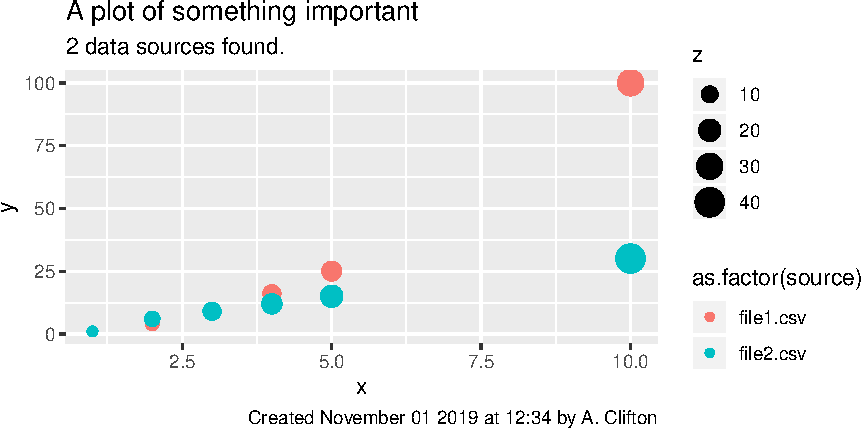
\includegraphics{main_files/figure-latex/plot-input-data-1.pdf}
\caption{\label{fig:plot-input-data}Input Data}
\end{figure}

I've used the \texttt{ggplot2} package to make this figure. This has the advantage that figures can be given a consistent look and feel through ggplot's themes.

For convenience, we'll also save a copy of the figure as a \emph{.png} file to the \texttt{output.dir} (\emph{analysis/}) directory.

\hypertarget{operate-on-the-data}{%
\subsection{Operate on the data}\label{operate-on-the-data}}

At this point we can do any number of operations on the data. For sake of demonstration, let's add 2 to all \(x\) values.

\begin{Shaded}
\begin{Highlighting}[]
\NormalTok{df.all <-}\StringTok{ }\NormalTok{df.in}
\NormalTok{df.all}\OperatorTok{$}\NormalTok{x <-}\StringTok{ }\NormalTok{df.in}\OperatorTok{$}\NormalTok{x }\OperatorTok{+}\StringTok{ }\FloatTok{2.0}
\end{Highlighting}
\end{Shaded}

\hypertarget{plot-the-results}{%
\subsection{Plot the results}\label{plot-the-results}}

Let's run that \texttt{plotSomething()} routine again.

\begin{figure}
\centering
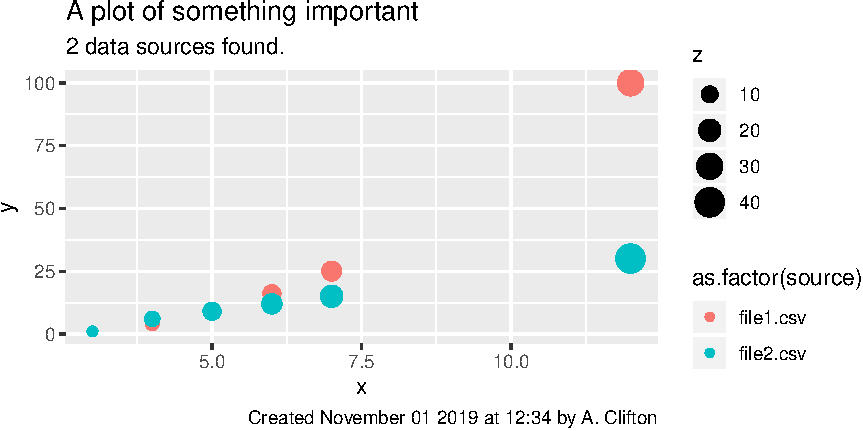
\includegraphics{main_files/figure-latex/plot-modified-data-1.pdf}
\caption{\label{fig:plot-modified-data}Modified Data}
\end{figure}

And, as we can see in Figure \ref{fig:plot-modified-data}, the data have shifted along \(x\) by a small amount.

\hypertarget{implementWrite}{%
\subsection{Write}\label{implementWrite}}

Writing in an R Markdown document is similar to most other types of markdown.

So far we have demonstrate that we can import and manipulate data and plot results. Another important part of a publication is the ability to generate statistics or summary information from data and include that in our text.

To demonstrate that, I can calculate that the maximum value of \(y\) in the input data sets was 100. This can be confirmed by checking the input data files. I could also include more complex logic in these statements, for example to say if one statistic is bigger or larger than another.

I can also include equations, and reference them (e.g.~Equation \eqref{eq:eq}). Markdown does not directly support equations, so we can be a bit flexible in notation. For simplicity in working with other parts of the workflow, I use Latex \texttt{begin\{equation\}...end\{equation\}} to indicate an equation.

\begin{equation}
A=\frac{\pi}{27d^2}
\label{eq:eq}
\end{equation}

This also works well with Word-format output.

You've already seen citations \citep{R-base}, which refers to bibtex entries in \href{main.bib}{\emph{main.bib}}. These first appeared in section \ref{sec:intro}. Footnotes work too.\footnote{See what I did there?}

We sometimes need to include formatted tables in documents. This can be done using the \texttt{kable()} function (Table \ref{tab:dfall}).

\begin{Shaded}
\begin{Highlighting}[]
\NormalTok{knitr}\OperatorTok{::}\KeywordTok{kable}\NormalTok{(df.all,}
  \DataTypeTok{format=}\StringTok{"pandoc"}\NormalTok{,}
  \DataTypeTok{caption =} \StringTok{"The _df.all_ data frame."}\NormalTok{)}
\end{Highlighting}
\end{Shaded}

\begin{longtable}[]{@{}rrrl@{}}
\caption{\label{tab:dfall}The \emph{df.all} data frame.}\tabularnewline
\toprule
x & y & z & source\tabularnewline
\midrule
\endfirsthead
\toprule
x & y & z & source\tabularnewline
\midrule
\endhead
3 & 1 & 3 & file1.csv\tabularnewline
4 & 4 & 6 & file1.csv\tabularnewline
5 & 9 & 9 & file1.csv\tabularnewline
6 & 16 & 12 & file1.csv\tabularnewline
7 & 25 & 15 & file1.csv\tabularnewline
12 & 100 & 30 & file1.csv\tabularnewline
3 & 1 & 4 & file2.csv\tabularnewline
4 & 6 & 8 & file2.csv\tabularnewline
5 & 9 & 12 & file2.csv\tabularnewline
6 & 12 & 16 & file2.csv\tabularnewline
7 & 15 & 20 & file2.csv\tabularnewline
12 & 30 & 40 & file2.csv\tabularnewline
\bottomrule
\end{longtable}

If our goal was just to produce HTML, we could add styling, too. This is detailed in the \emph{kable} package vignettes.\footnote{In this example I have explicitly stated \texttt{\_format="pandoc"\_} so that this file will work in HTML and PDF.}

\hypertarget{implementSave}{%
\subsection{Save}\label{implementSave}}

We now write our processed data to file.

\begin{Shaded}
\begin{Highlighting}[]
\CommentTok{# save the data}
\KeywordTok{save}\NormalTok{(}\DataTypeTok{list =} \KeywordTok{c}\NormalTok{(}\StringTok{"base.dir"}\NormalTok{,}
              \StringTok{"made.by"}\NormalTok{,}
              \StringTok{"df.all"}\NormalTok{),}
       \DataTypeTok{file =} \KeywordTok{file.path}\NormalTok{(base.dir, output.dir, }\StringTok{"Data.RData"}\NormalTok{),}
       \DataTypeTok{envir =}\NormalTok{ .GlobalEnv)}
\end{Highlighting}
\end{Shaded}

In R it is also possible to save the whole workspace. We can do that here as well:

\begin{Shaded}
\begin{Highlighting}[]
\CommentTok{# save the workspace}
\KeywordTok{save.image}\NormalTok{(}\DataTypeTok{file=}\KeywordTok{file.path}\NormalTok{(base.dir, output.dir,}\StringTok{"workspace.RData"}\NormalTok{))}
\end{Highlighting}
\end{Shaded}

\hypertarget{implementIterate}{%
\subsection{Iterate}\label{implementIterate}}

To re-run the analysis, render \emph{main.rmd} every so often following the instructions in \emph{HOWTO.md}.

Some IDEs also allow the code chunks to be evaluated separately, which might help when dealing with larger data sets, more complex analysis, or bigger documents.

\hypertarget{implementFformat}{%
\subsection{Apply formatting}\label{implementFformat}}

Scientific Journals often have their own formatting requirements. These requirements can still be met using markdown. The mechanics of such a process are beyond the scope of this paper and should probably be done as the last step in the publishing process. The reader is encouraged to look at the \href{https://github.com/rstudio/rticles}{\emph{rticles}} package and to use the detailed instructions in section 13 of the R Markdown Guide \citep{R-Markdown-Guide}.

\hypertarget{does-this-approach-lead-to-reproducable-research}{%
\section{Does this approach lead to reproducable research?}\label{does-this-approach-lead-to-reproducable-research}}

If you would like to test the reproducibility of this approach, try this:

\begin{enumerate}
\def\labelenumi{\arabic{enumi}.}
\tightlist
\item
  Make sure you have set up the computing environment.
\item
  Make a copy of the entire working directory. Put that somewhere safe.
\item
  In the working directory, remove the results:

  \begin{enumerate}
  \def\labelenumii{\arabic{enumii}.}
  \tightlist
  \item
    Delete the \emph{analysis} directory.
  \item
    Delete the \emph{publications/} directory and all of its subdirectories. This is where \emph{main.PDF}, \emph{main.html}, and \emph{main.md} are.
  \end{enumerate}
\end{enumerate}

You should now be left with some raw data and a few codes. There's no documentation anymore and no results.

\begin{enumerate}
\def\labelenumi{\arabic{enumi}.}
\setcounter{enumi}{4}
\tightlist
\item
  Render \emph{main.rmd}. There are instructions on how to do this in the \emph{HOWTO.md} file included in the root directory of the repository.
\end{enumerate}

You now should have your data folder back and all of the documentation, but you'll notice that the dates on the figures might have changed. This is reproducable research in action.

\hypertarget{r5}{%
\subsubsection{R\^{}5}\label{r5}}

\begin{quote}
``need to finish this''
\end{quote}

\hypertarget{is-this-fair}{%
\subsection{Is this FAIR?}\label{is-this-fair}}

``FAIR'' data stands for data that are Findable, Accessible, Interoperable, and Reusable.

\begin{quote}
``need to finish this''
\end{quote}

\hypertarget{findable}{%
\subsubsection{Findable}\label{findable}}

\hypertarget{accesible}{%
\subsubsection{Accesible}\label{accesible}}

\hypertarget{interoperable-data}{%
\subsubsection{Interoperable data}\label{interoperable-data}}

Our data were stored as comma-separated values in .csv files. These are not ideal; besides the meaningless column headers, there's no metadata. Instead, it would have been better if the data had been in a relevant, \texttt{standardized} format that included metadata in the headers. An even better solution would be a self-describing format that includes metadata for all of the included fields.

\hypertarget{reusable}{%
\subsubsection{Reusable}\label{reusable}}

\hypertarget{making-the-results-portable}{%
\subsection{Making the results portable}\label{making-the-results-portable}}

One way to ensure repeatability and reproducability may be to have a generic ``data processing'' image of a computer system, e.g.~as a Docker image, that is started for each new project and used \emph{only} for that project. This clean system is then used for one data processing task which is managed through a file such as the one you are reading. When the project is complete, the image is simply stored for as long as required. This would also avoid problems associated with changes introduced by package and system updates. A drawback to this approach would be the need to migrate the data every 5 years or so to a new system, which would be required to avoid data being stranded on old software.

\begin{quote}
``need to finish this''
\end{quote}

\hypertarget{conclusions}{%
\section{Conclusions}\label{conclusions}}

Literate programming allows the creation of a single document that captures all of the process of preparing and analysing data, and creating a publication to describe that data. This is a fundamental requirement of reproducible research.

\hypertarget{referencing-this-document}{%
\section*{Referencing this document}\label{referencing-this-document}}
\addcontentsline{toc}{section}{Referencing this document}

This document has been assigned the Digital Object Identifier \href{http://dx.doi.org/10.5281/zenodo.3497450}{10.5281/zenodo.3497450}. Citations in a range of formats can be obtained through Zenodo.

\href{https://doi.org/10.5281/zenodo.3497450}{
\includegraphics{DOIBadge3497450.pdf}}

The source code for this document is available through \href{https://github.com/AndyClifton/lit-pro-sci-pub-demo}{github.com/AndyClifton/lit-pro-sci-pub-demo}.

\hypertarget{acknowledgements}{%
\section*{Acknowledgements}\label{acknowledgements}}
\addcontentsline{toc}{section}{Acknowledgements}

Many thanks to Nikola Vasiljevic at DTU for prompting me to get this done.

\renewcommand\refname{Bibliography}
\bibliography{main.bib}


\end{document}
